\documentclass{beamer}
\usetheme{Madrid}
\usecolortheme{default}

\usepackage{tikz}
\usepackage{pgfplots}
\usetikzlibrary{shapes, arrows, positioning, calc, backgrounds, shadows}
\pgfplotsset{compat=1.18}

% --- TikZ Styles ---
\tikzstyle{block} = [rectangle, draw, fill=blue!20, text width=5em, text centered, rounded corners, minimum height=3em, drop shadow]
\tikzstyle{line} = [draw, -latex']
\tikzstyle{cloud} = [draw, ellipse, fill=red!20, node distance=3cm, minimum height=2em]
\tikzstyle{code} = [rectangle, draw=black!50, fill=gray!10, font=\ttfamily\scriptsize, align=left]

\title{Benchmarking JAX for Molecular Scoring}
\subtitle{JIT Compilation, Warmup, and GPU Synchronization}
\author{Expert Assistant}
\date{\today}

\begin{document}

% Slide 1: Title
\begin{frame}
    \titlepage
\end{frame}

% Slide 2: What is JAX? (Visual Flow)
\begin{frame}{What is JAX actually doing?}
    \begin{columns}
        \column{0.4\textwidth}
        \textbf{Core Concepts:}
        \begin{itemize}
            \item \textbf{Transformation:} Python $\to$ Abstract Syntax Tree.
            \item \textbf{Vectorization:} \texttt{vmap} replaces loops.
            \item \textbf{XLA:} Fuses operations to minimize memory access.
        \end{itemize}

        \column{0.6\textwidth}
        \centering
        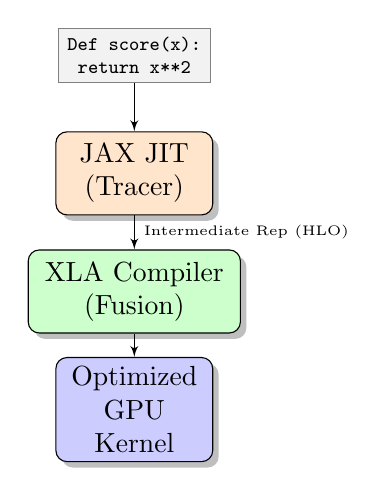
\begin{tikzpicture}[node distance = 1.5cm, auto]
            % Nodes
            \node [code] (python) {Def score(x):\\ \ return x**2};
            \node [block, below of=python, fill=orange!20] (jit) {JAX JIT\\(Tracer)};
            \node [block, below of=jit, fill=green!20, text width=7em] (xla) {XLA Compiler\\(Fusion)};
            \node [block, below of=xla, fill=blue!20] (gpu) {Optimized GPU Kernel};

            % Lines
            \path [line] (python) -- (jit);
            \path [line] (jit) -- node[right, font=\tiny]{Intermediate Rep (HLO)} (xla);
            \path [line] (xla) -- (gpu);
        \end{tikzpicture}
    \end{columns}
\end{frame}

% Slide 3: JIT vs Interpreter (Visual Comparison)
\begin{frame}[fragile]{Just-In-Time (JIT) Compilation}
    \textbf{Why JIT?} Avoids the overhead of Python's interpreter loop.

    \vspace{0.5cm}

    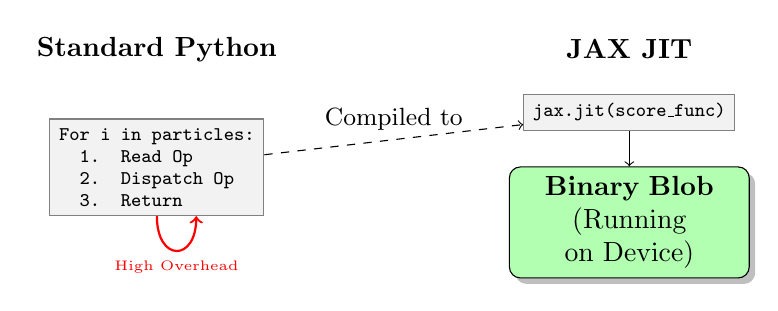
\begin{tikzpicture}
        % Left Side: Python
        \node (py_label) at (0, 3) {\textbf{Standard Python}};
        \node[code] (py_loop) at (0, 1.5) {
            For i in particles:\\
            \ \ 1. Read Op\\
            \ \ 2. Dispatch Op\\
            \ \ 3. Return
        };
        \draw[->, thick, red] ($(py_loop.south)+(0,0)$) to[out=270,in=270, looseness=3] node[below, font=\tiny, red]{High Overhead} ($(py_loop.south)+(0.5,0)$);

        % Right Side: JAX
        \node (jax_label) at (6, 3) {\textbf{JAX JIT}};
        \node[code] (jax_code) at (6, 2.2) {jax.jit(score\_func)};
        \node[block, fill=green!30, text width=8em] (binary) at (6, 0.8) {\textbf{Binary Blob}\\(Running on Device)};
        
        \draw[->, dashed] (py_loop) -- node[above, font=\small]{Compiled to} (jax_code);
        \draw[->] (jax_code) -- (binary);
    \end{tikzpicture}
    
    \vspace{0.2cm}
    \footnotesize
    Code: \texttt{jax\_ev\_jit = jax.jit(jax\_excluded\_volume)}
\end{frame}

% Slide 4: Warmup (Chart)
\begin{frame}{The Necessity of "Warmup" Runs}
    \textbf{Problem:} The first run triggers compilation (very slow).
    
    \begin{center}
    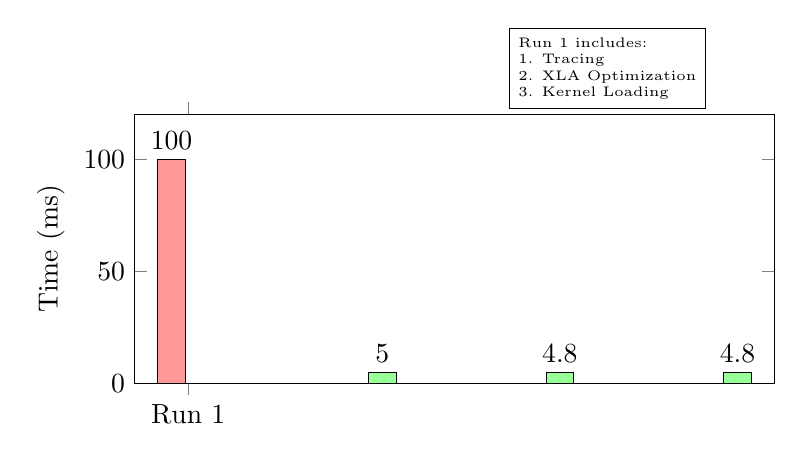
\begin{tikzpicture}
        \begin{axis}[
            ybar,
            symbolic x coords={Run 1, Run 2, Run 3, Run 4},
            xtick=data,
            ylabel={Time (ms)},
            nodes near coords,
            ymin=0, ymax=120,
            width=0.8\textwidth,
            height=5cm
        ]
            % The Compilation Spike
            \addplot[fill=red!40] coordinates {(Run 1, 100)};
            % The Actual Speed
            \addplot[fill=green!40] coordinates {(Run 2, 5) (Run 3, 4.8) (Run 4, 4.8)};
        \end{axis}
        
        % Annotations
        \node[draw, align=left, font=\tiny] at (6, 4) {Run 1 includes:\\1. Tracing\\2. XLA Optimization\\3. Kernel Loading};
    \end{tikzpicture}
    \end{center}
    
    \begin{itemize}
        \item \textbf{Strategy:} Run 5 "throwaway" loops first.
        \item \textbf{Goal:} Ensure kernels are cached and GPU is initialized.
    \end{itemize}
\end{frame}

% Slide 5: Async Execution (Timeline)
\begin{frame}{CPU-GPU Synchronization}
    JAX is \textbf{Asynchronous}. The CPU dispatches work and moves on.

    \vspace{0.5cm}
    \centering
    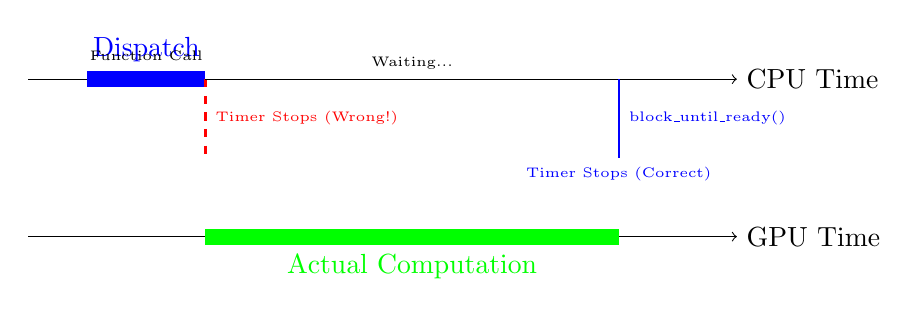
\begin{tikzpicture}[xscale=1.5]
        % Swimlanes
        \draw[->] (0, 2) -- (6, 2) node[right] {CPU Time};
        \draw[->] (0, 0) -- (6, 0) node[right] {GPU Time};

        % CPU Events
        \fill[blue] (0.5, 1.9) rectangle (1.5, 2.1) node[midway, above=0.1cm] {Dispatch};
        \node[font=\tiny] at (1.0, 2.3) {Function Call};

        % GPU Events
        \fill[green] (1.5, -0.1) rectangle (5.0, 0.1) node[midway, below=0.1cm] {Actual Computation};

        % Scenario A: No Block
        \draw[red, dashed, thick] (1.5, 2) -- (1.5, 1) node[midway, right, font=\tiny] {Timer Stops (Wrong!)};
        
        % Scenario B: With Block
        \draw[dotted] (1.5, 2) -- (5.0, 2) node[midway, above, font=\tiny] {Waiting...};
        \draw[blue, thick] (5.0, 2) -- (5.0, 1) node[midway, right, font=\tiny] {block\_until\_ready()};
        \node[font=\tiny, text=blue] at (5.0, 0.8) {Timer Stops (Correct)};

    \end{tikzpicture}

    \vspace{0.5cm}
    \begin{itemize}
        \item Without \texttt{.block\_until\_ready()}, we only measure the dispatch time ($\sim \mu s$).
        \item With blocking, we measure the math ($\sim ms$).
    \end{itemize}
\end{frame}

% Slide 6: Summary Methodology (Flowchart)
\begin{frame}{Benchmark Methodology Pipeline}
    
    \begin{center}
    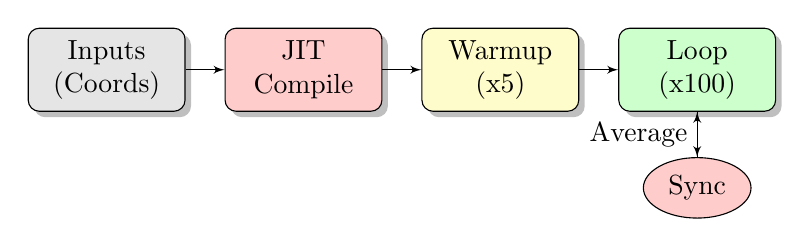
\begin{tikzpicture}[node distance=2.5cm, auto]
        \node [block, fill=gray!20] (input) {Inputs\\(Coords)};
        \node [block, right of=input, fill=red!20] (compile) {JIT\\Compile};
        \node [block, right of=compile, fill=yellow!20] (warmup) {Warmup\\(x5)};
        \node [block, right of=warmup, fill=green!20] (loop) {Loop\\(x100)};
        \node [cloud, below of=loop, node distance=1.5cm] (sync) {Sync};
        
        \path [line] (input) -- (compile);
        \path [line] (compile) -- (warmup);
        \path [line] (warmup) -- (loop);
        \path [line] (loop) -- (sync);
        \path [line] (sync) -- node[left] {Average} (loop); % Representing the loop logic visually
    \end{tikzpicture}
    \end{center}

    \begin{enumerate}
        \item \textbf{Consistency:} Identical particles for all backends.
        \item \textbf{Stability:} Warmup eliminates compilation noise.
        \item \textbf{Accuracy:} \texttt{block\_until\_ready()} captures hardware reality.
    \end{enumerate}
\end{frame}
%
\begin{frame}
\begin{figure}
    \centering
    \includegraphics[width=0.7\textwidth]{figures/benchmark_results.png}
\end{figure}
\end{frame}
%
\end{document}